% Yale University Poster - Gemini Theme
% Serial Dilution Ecological Modeling Project

\documentclass[final]{beamer}

% ====================
% Packages
% ====================

\usepackage[T1]{fontenc}
\usepackage{lmodern}
\usepackage[size=custom, width=122, height=91, scale=1.2]{beamerposter}
\usetheme{gemini}
\usecolortheme{msu}
\usepackage{graphicx}
\usepackage{booktabs}
\usepackage{tikz}
\usepackage{pgfplots}
\pgfplotsset{compat=1.14}
\usepackage{anyfontsize}
\usepackage{amsmath}
\usepackage{amssymb}

% ====================
% Lengths
% ====================

% (3 columns) + 4 separators = paperwidth
% 4 * 0.025 + 3 * 0.30 = 0.10 + 0.90 = 1.00
\newlength{\sepwidth}
\newlength{\colwidth}
\setlength{\sepwidth}{0.025\paperwidth}
\setlength{\colwidth}{0.30\paperwidth}

\newcommand{\separatorcolumn}{\begin{column}{\sepwidth}\end{minipage}\egroup\typeout{MEASURED_COL_HEIGHT: \the\ht0}}

% ====================
% Title & Authors
% ====================

\title{A Universal Physical Consumer-Resource Neural ODE Framework for Microbial Serial Dilution Ecology}

\author{Karthik Srinivasan\textsuperscript{1}, Germ\'an Plata\textsuperscript{2}, Purushottam Dixit\textsuperscript{1}}

\institute[shortinst]{\textsuperscript{1}Department of Biomedical Engineering, Yale University \samelineand \textsuperscript{2}Computational Sciences, BiomEdit, LLC.}

% ====================
% Footer & Logos
% ====================

\footercontent{
  \textbf{Cross-Dataset Benchmarks:} Venturelli et al. (\textit{MSB} 2018) \;\textbullet\; Pollard et al. (\textit{Nat. Commun.} 2023) \;\textbullet\; German et al. (Rumen) \;\textbullet\; Gore et al. (\textit{Science} 2022)
  \hfill
  \href{mailto:karthik.srinivasan@yale.edu}{karthik.srinivasan@yale.edu}
}

\logoleft{
\includegraphics[height=6.0cm]{logos/logo.png}}
\logoright{
\includegraphics[height=5.2cm]{figures/attribution_and_qr.png}}

% ====================
% Document Body
% ====================

\begin{document}

\begin{frame}[t]
\begin{columns}[t]
\separatorcolumn

% ════════════════════════════════════════════════════════════════════════════════
% COLUMN 1: Foundations & Out-of-Sample Generalization (Ophelia)
% ════════════════════════════════════════════════════════════════════════════════
\setbox0=\vbox\bgroup\begin{minipage}{\colwidth}

  % 1. BACKGROUND & DILEMMA
  \begin{block}{1. Background: Serial Dilution Regimes \& Modeling Dilemma}
    \begin{itemize}
      \item \textbf{Serial Dilution Ecology:} Cycles of continuous intra-cycle nutrient uptake and metabolic interaction interrupted by periodic discrete dilution ($1:D$) and dispersal ($\mu$).
      \item \textbf{Why Generalized Lotka-Volterra (gLV) Fails:} Requires $N^2$ empirical interaction coefficients, assumes fixed interaction signs, cannot model substrate depletion, and overfits severely ($N=48$ requires $2{,}304$ parameters).
      \item \textbf{The Simplex Reset Artifact:} Normalizing relative abundances to $\sum x_i = 1$ at transfers mutes quadratic self-limitation ($-\alpha_i N_i^2$) and triggers artificial competitive exclusion cascades.
    \end{itemize}
  \end{block}

  % 2. PHYSICAL NEURAL ODE FORMULATION
  \begin{block}{2. Physical Consumer-Resource Neural ODE Formulation}
    We model continuous within-passage growth coupled to discrete dilution transfers:
    \begin{align*}
      \frac{dN_i}{dt} &= N_i(t) \left( \sum_{k=1}^K \Theta_{ik} R_k(t) \right) - \alpha_i N_i(t)^2 \\
      \frac{dR_k}{dt} &= - R_k(t) \left[ \sum_{i=1}^N \Theta_{ik} N_i(t) - \sum_{l=1}^K W_{lk} \left( \sum_{j=1}^N \Theta_{jl} N_j(t) \right) \right]
    \end{align*}
    \begin{itemize}
      \item \textbf{Physical Parameter Constraints:} $\Theta \ge 0$ (uptake traits), $W \ge 0$ (byproduct cross-feeding), $\alpha > 0$ (self-limitation / crowding), $R_0 = \text{softplus}(\mathbf{a}_c) \ge 0$.
      \item \textbf{Physical Continuity Across Passages ($m \to m+1$):}
        $N_i(0)^{(m+1)} = \frac{N_i(\tau)^{(m)}}{D} + \mu \cdot M_{c, i}, \quad R_k(0)^{(m+1)} = R_{0, c, k}$. Eliminates simplex resets.
      \item \textbf{Closed-Form Effective Interaction Operator:}
        \begin{equation*}
          \mathbf{A}^{(c)} = -\text{diag}(\mathbf{\alpha}) - \kappa \, \mathbf{\Theta} \, \text{diag}(\mathbf{R}_{0, c}) \, (\mathbf{I} - \mathbf{W})^T \mathbf{\Theta}^T
        \end{equation*}
        Decomposes into intra-specific crowding ($-\alpha$), niche competition ($-\mathbf{\Theta}\mathbf{R}_0\mathbf{\Theta}^T$), and facilitation ($+\mathbf{\Theta}\mathbf{R}_0\mathbf{W}^T\mathbf{\Theta}^T$). Shows rank $\le K \ll N$.
    \end{itemize}
  \end{block}

  % 3. HELD-OUT GENERALIZATION: OPHELIA
  \begin{block}{3. Out-of-Sample Generalization: Venturelli et al. (2018)}
    \begin{itemize}
      \item \textbf{Held-Out Test Consortia:} 73 complex synthetic human gut communities ($4{,}380$ dynamic points) never seen during model training.
      \item \textbf{Minimal Validation Loss Architecture ($K=7$):} Optimal trade-off between expressive capacity and generalization ($\mathcal{L}_{\text{GKL}} = \mathbf{0.12950}$).
    \end{itemize}

    \begin{figure}
      \centering
      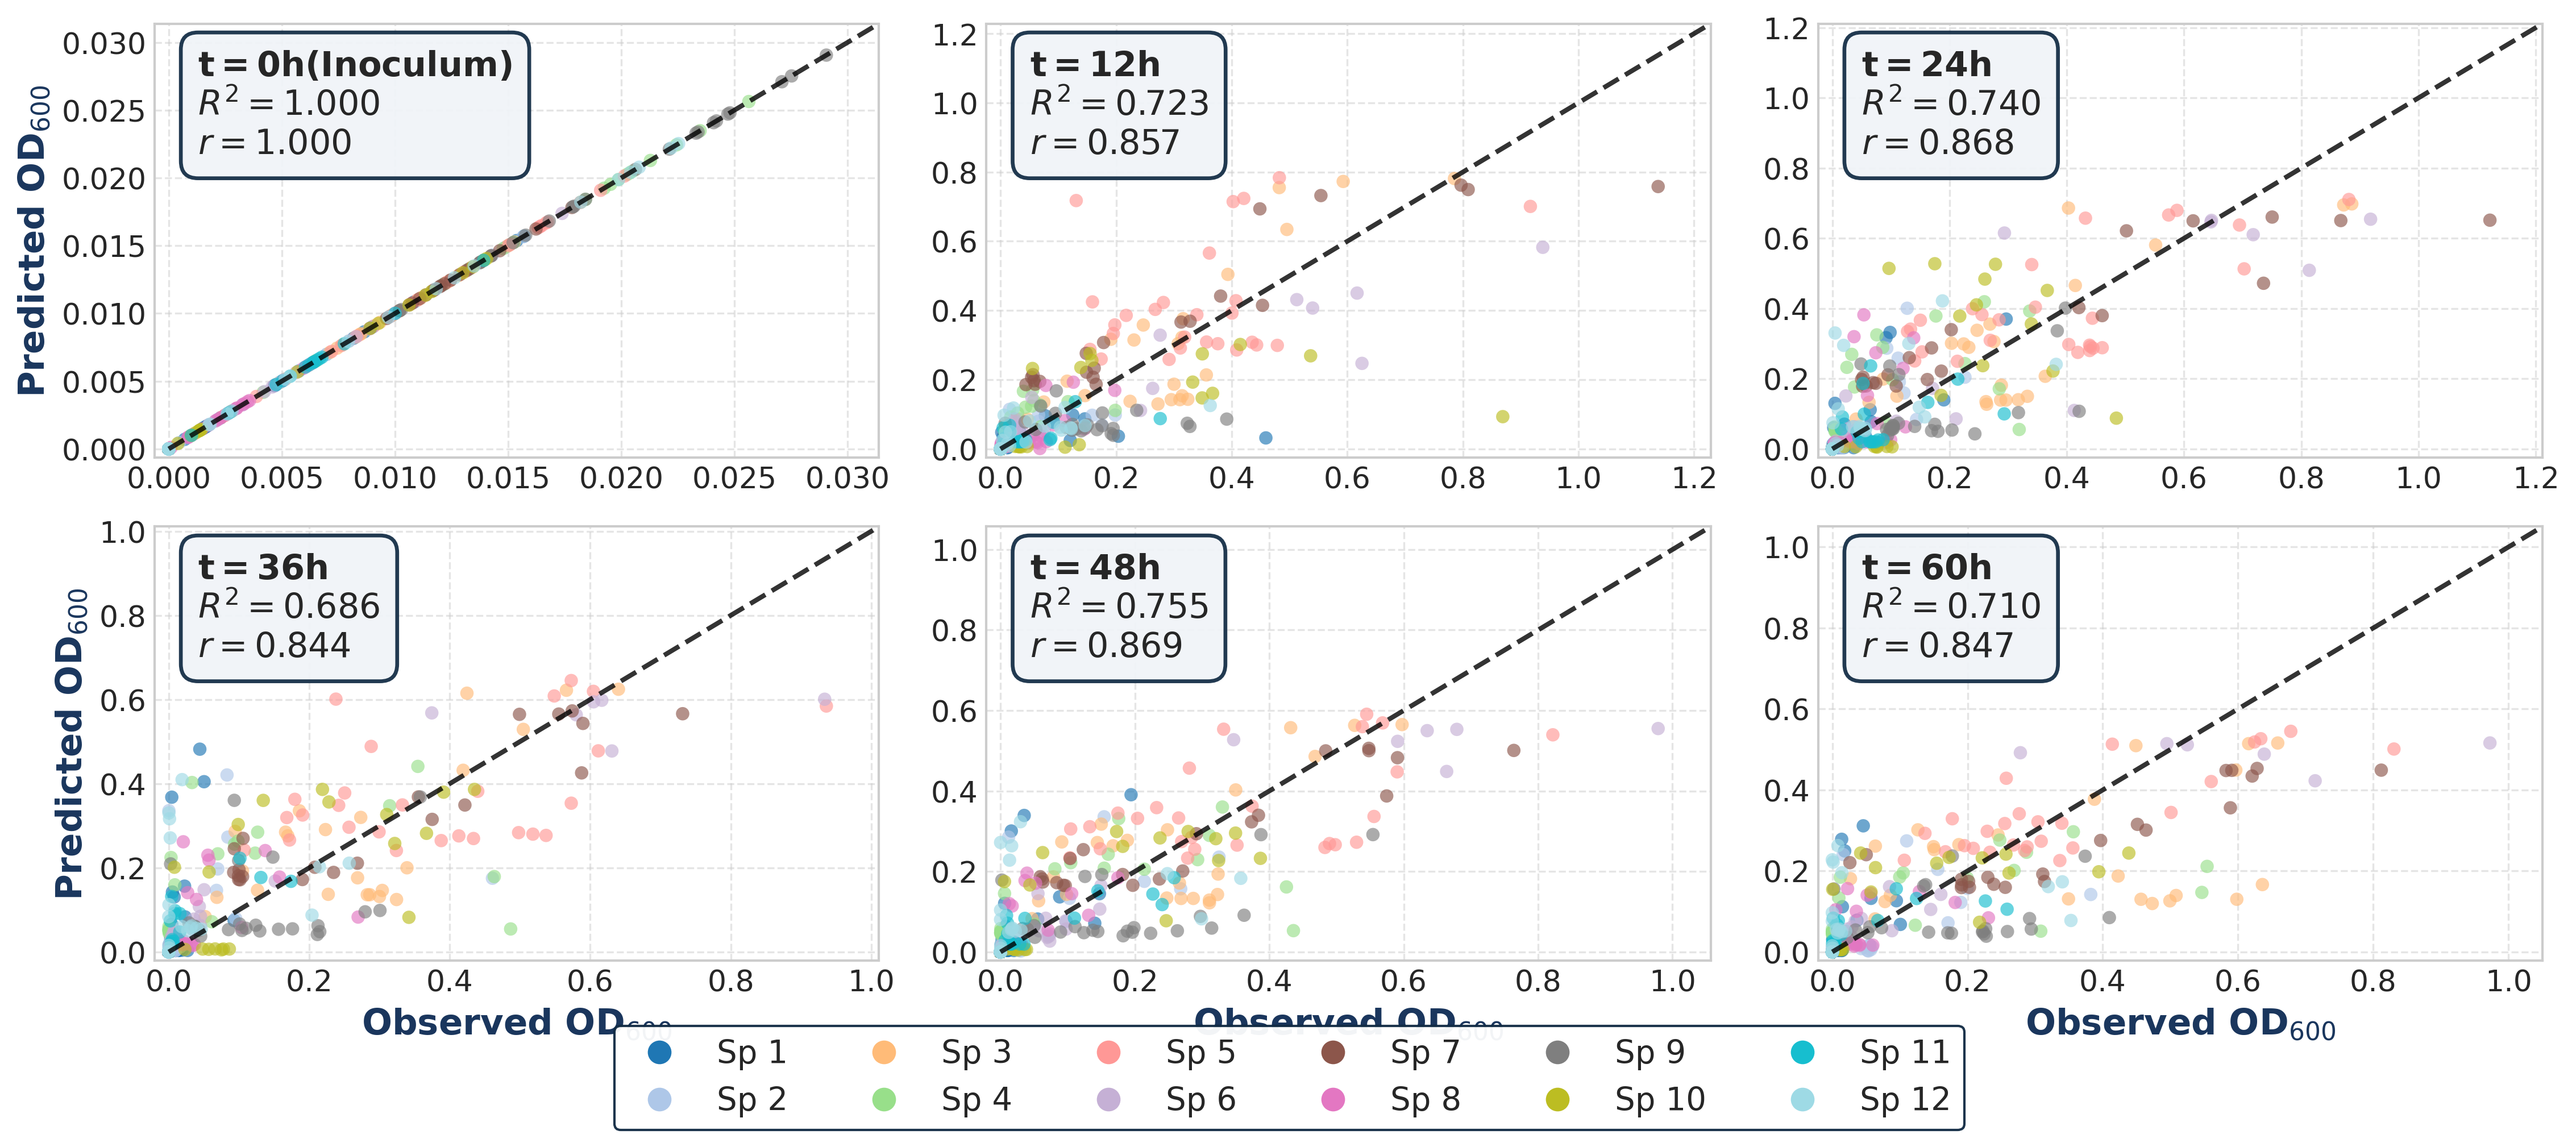
\includegraphics[width=0.98\linewidth]{figures/Ophelia_Test_Scatter.png}
      \caption{\textbf{Six-Panel Held-Out Generalization Across Time ($t=12n$, $n=0\dots5$).} Observed vs. predicted absolute biomass ($OD_{600}$) across 73 unseen gut communities and 12 species from $t=0\text{h}$ to $60\text{h}$ ($R^2 = \mathbf{0.69\text{--}0.75}$, Pearson $r = \mathbf{0.84\text{--}0.87}$ across dynamic timepoints; overall test $R^2 = \mathbf{0.7233}$, $\log_{10} r = \mathbf{0.9652}$, Spearman $\rho = \mathbf{0.9901}$).}
    \end{figure}
  \end{block}

\end{minipage}\egroup\typeout{MEASURED_COL_HEIGHT: \the\ht0}

\separatorcolumn

% ════════════════════════════════════════════════════════════════════════════════
% COLUMN 2: Universality (Pollard) & Environmental Specificity (German)
% ════════════════════════════════════════════════════════════════════════════════
\setbox0=\vbox\bgroup\begin{minipage}{\colwidth}

  % 4. UNIVERSALITY: POLLARD
  \begin{block}{4. Universality of Metabolic Trait Matrices: Pollard et al. (2023)}
    \begin{itemize}
      \item \textbf{Spatial Carrier Microenvironments:} 50 human gut isolates transferred across 5 carriers: Liquid broth, Mucin carriers, Plain agar, and Supernatants.
      \item \textbf{Universal Invariant Traits:} A single metabolic uptake matrix $\mathbf{\Theta}$ ($50 \times 5$) and cross-feeding matrix $\mathbf{W}$ ($5 \times 5$) govern all 5 environments. Carrier divergence is controlled strictly by the learned environmental vector $\mathbf{a}_c \in \mathbb{R}^5$.
      \item \textbf{Spatial Refugia Prevent Washout:} Solid carriers stably preserve $\mathbf{21\text{--}24}$ \textbf{species} ($\exp(H) \approx 11\text{--}15$) over 100 serial passages by sheltering sensitive taxa, whereas liquid broth collapses to $11.0$ species ($\exp(H) = 5.44$).
    \end{itemize}

    \begin{figure}
      \centering
      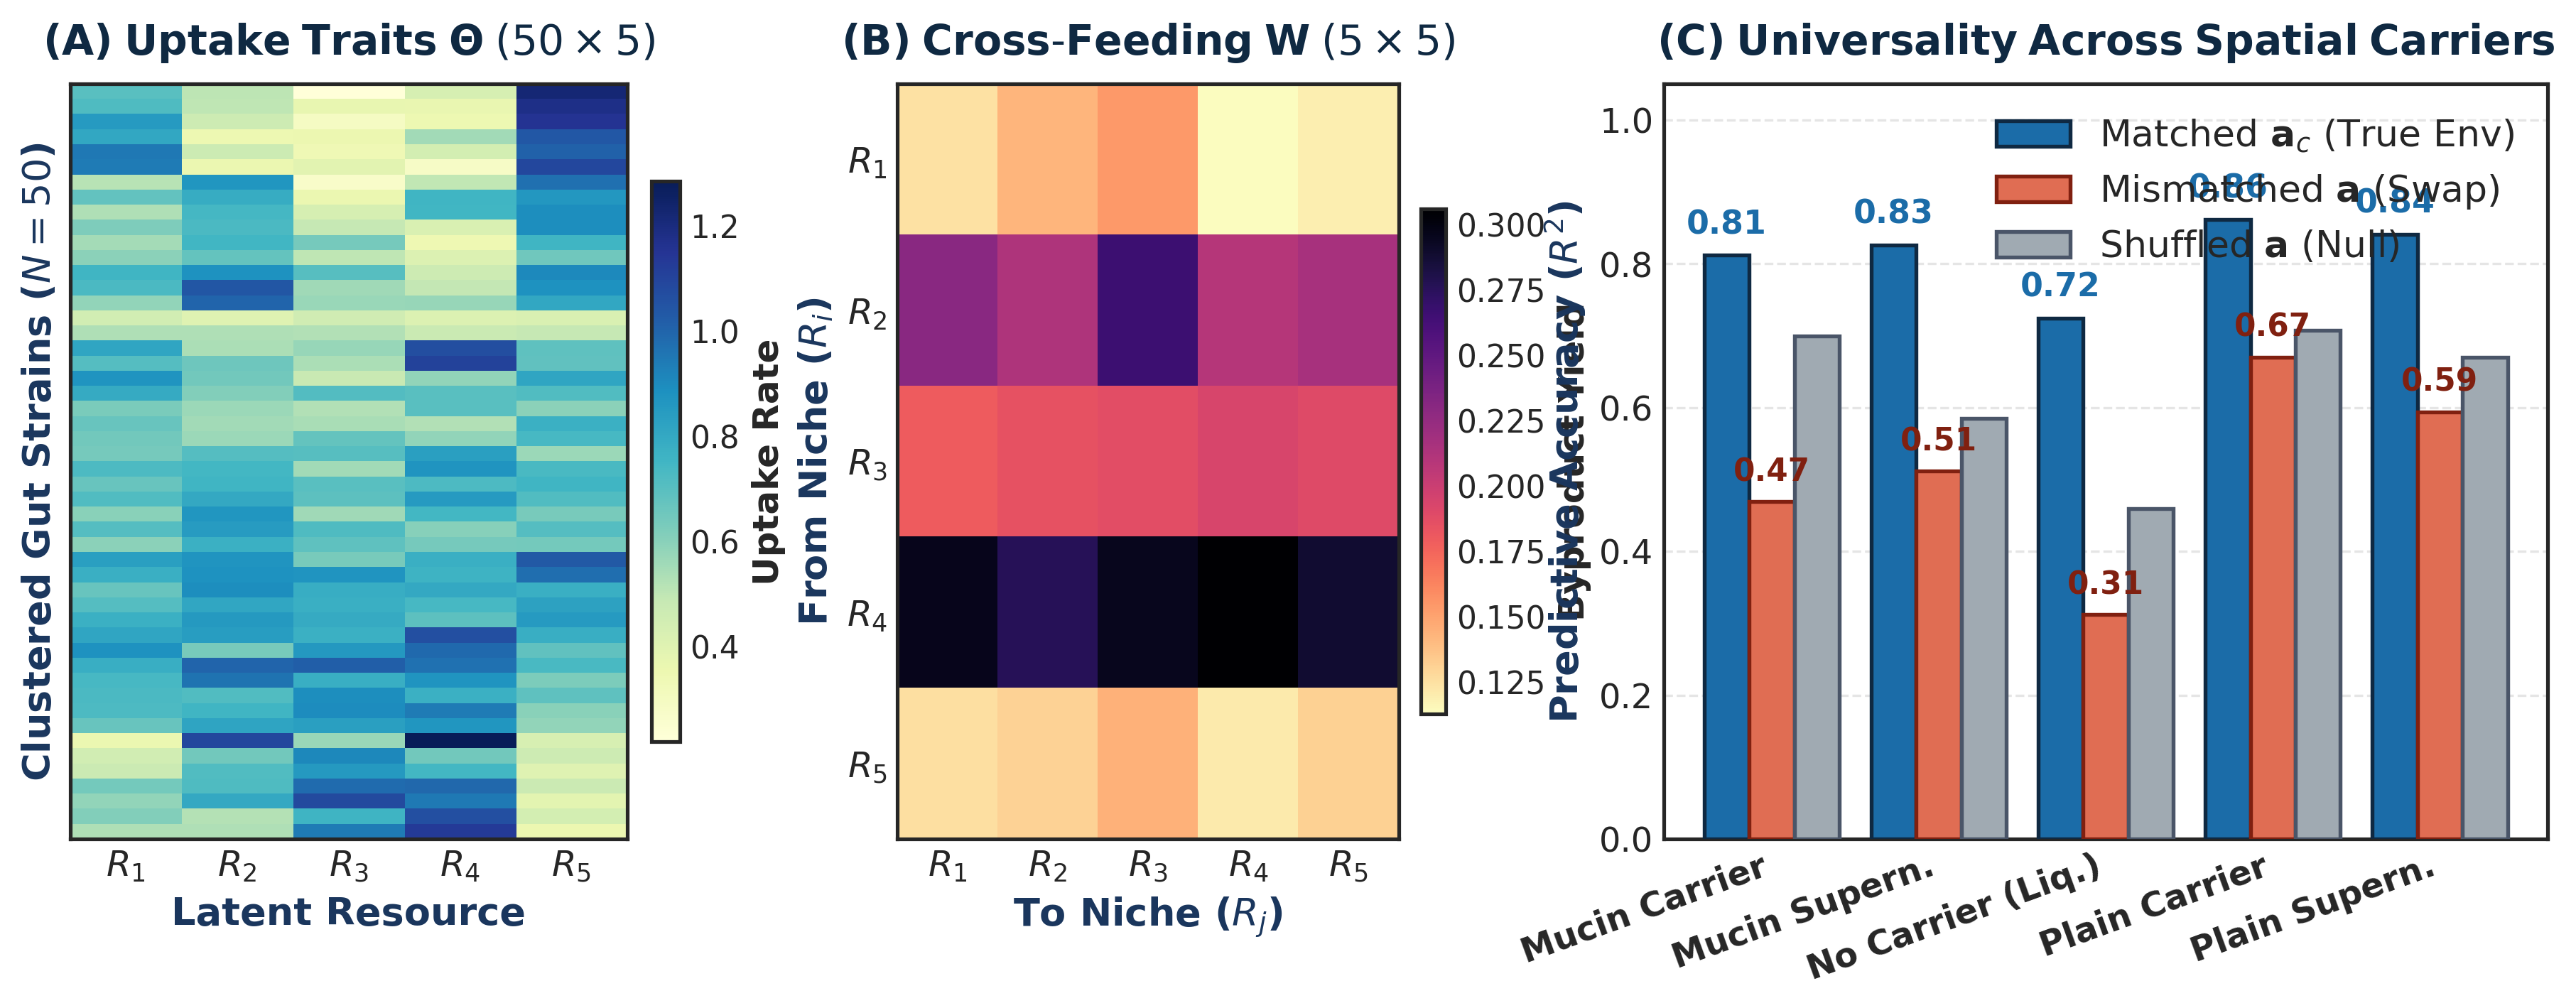
\includegraphics[width=0.98\linewidth]{figures/Pollard_Universal_Matrices.png}
      \caption{\textbf{Universality Across 5 Spatial Microenvironments.} \textbf{(A)} Clustered uptake traits $\mathbf{\Theta}$ reveal specialized metabolic guilds. \textbf{(B)} Cross-feeding byproduct matrix $\mathbf{W}$. \textbf{(C)} Matched $\mathbf{a}_c$ achieves $R^2 = \mathbf{0.725\text{--}0.862}$ (mean $\mathbf{0.813}$), whereas carrier swaps ($R^2 = 0.511$) and shuffled nulls ($R^2 = 0.580$) collapse.}
    \end{figure}
  \end{block}

  % 5. ENVIRONMENTAL SPECIFICITY: GERMAN
  \begin{block}{5. Meaningful Environmental Vectors: German et al. (Rumen)}
    \begin{itemize}
      \item \textbf{Longitudinal Methanogen Recovery ($N=91$ Strains, Peak $\ge 1\%$):} Retains $\mathbf{22}$ \textbf{methanogenic archaea} capturing $\mathbf{98.5\%}$ of archaeal reads and $\mathbf{92.3\%}$ of total community coverage across 6 geochemical perturbations.
      \item \textbf{Environmental Specificity vs. Severe Null Collapse:} True learned $\mathbf{a}$ achieves $\mathbf{R^2 = 0.8224}$ (Pearson $\mathbf{r = 0.9074}$, $\mathcal{L}_{\text{KL}} = \mathbf{1.7128}$ at $K=12$). Condition swaps cause a $\mathbf{59.7\%}$ collapse in accuracy ($R^2 = 0.3313$), while shuffling $\mathbf{a}$ completely destroys predictive ability ($R^2 = -1.1257$).
    \end{itemize}

    \begin{figure}
      \centering
      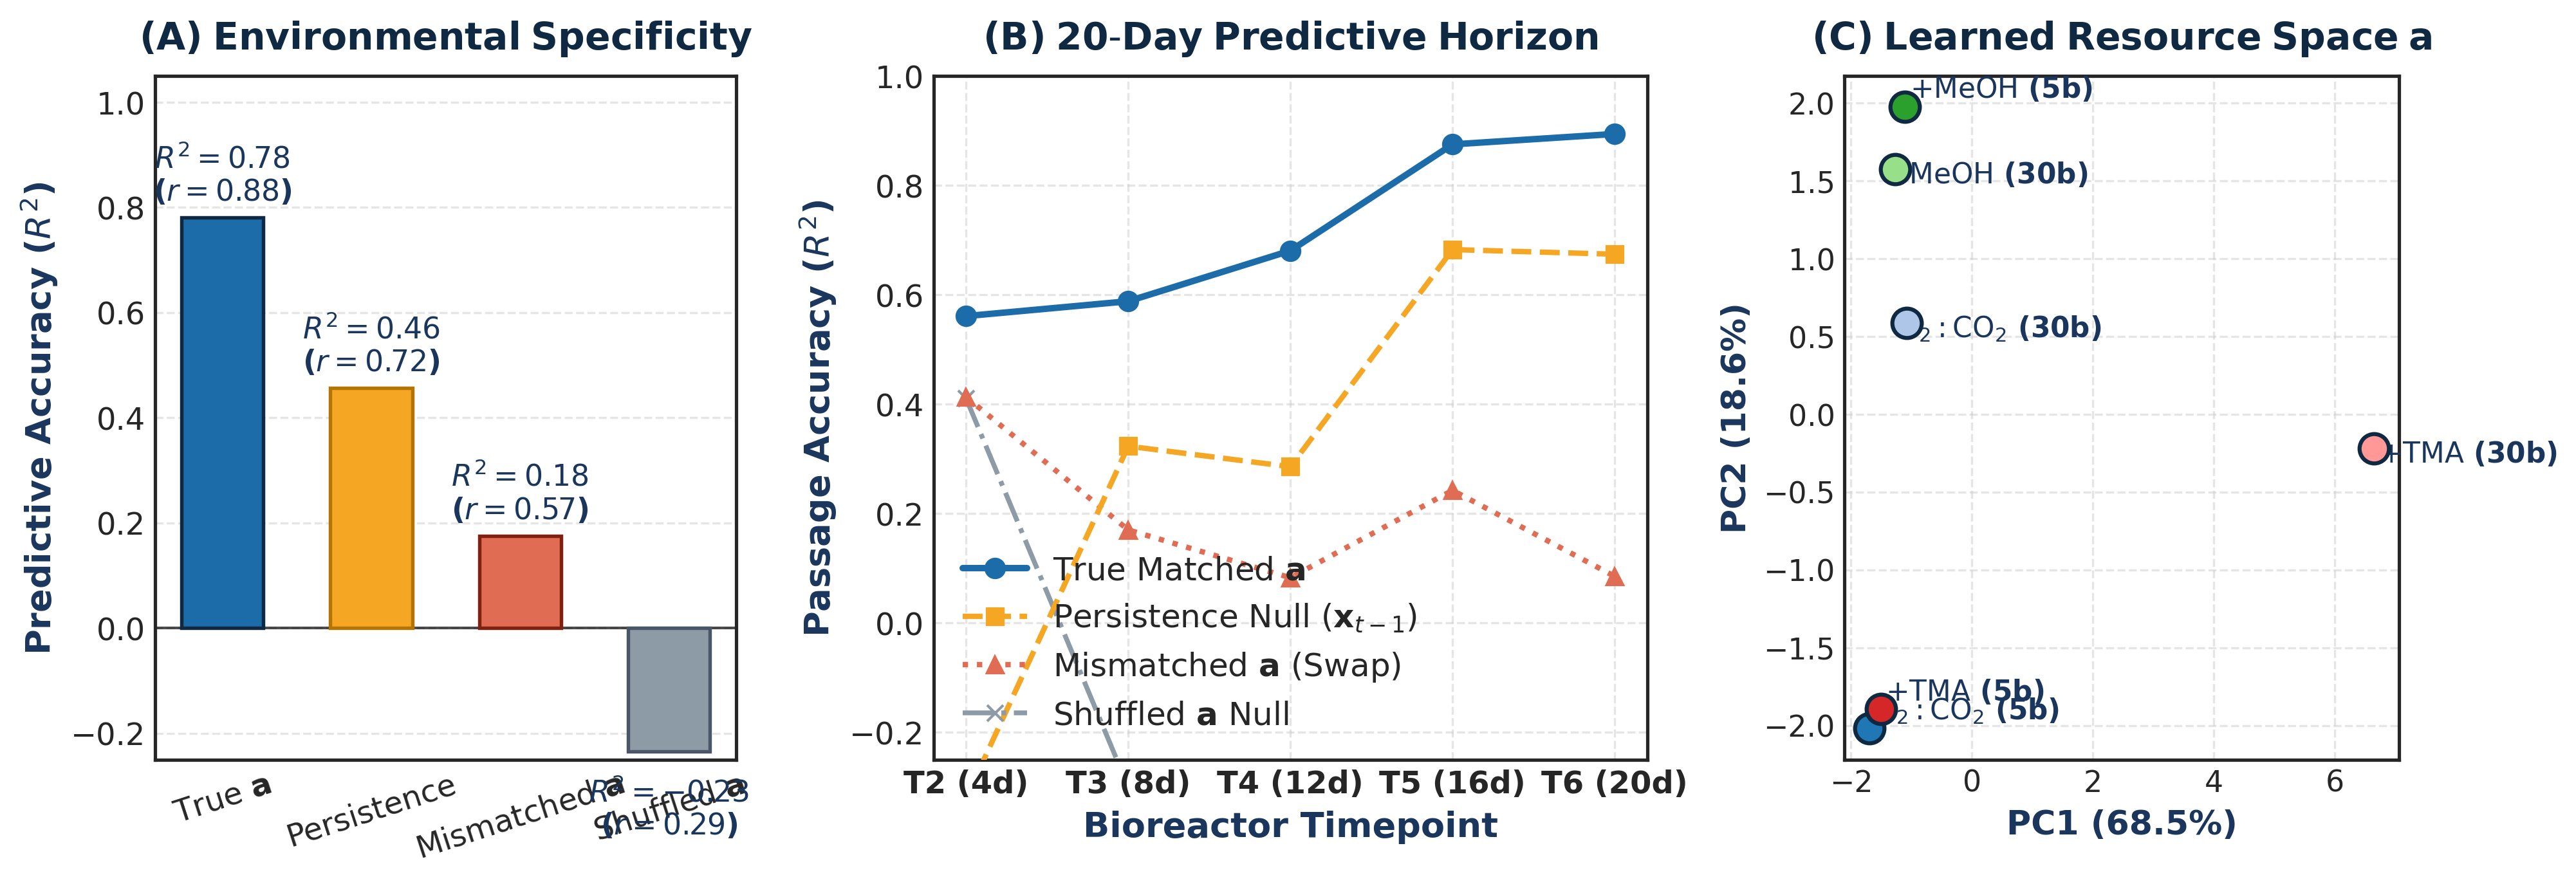
\includegraphics[width=0.98\linewidth]{figures/German_A_Vector_Null_Comparison.png}
      \caption{\textbf{Environmental Specificity vs. Null Baselines.} \textbf{(A)} True learned $\mathbf{a}$ ($R^2 = \mathbf{0.822}$, $r = \mathbf{0.907}$) significantly outperforms persistence null ($R^2 = 0.559$), mismatched conditions ($R^2 = 0.331$), and shuffled null ($R^2 = -1.13$). \textbf{(B)} Multi-passage horizon stability over 20 days. \textbf{(C)} PCA of learned $\mathbf{a}$ vectors autonomously clusters substrate and pressure chemistry.}
    \end{figure}
  \end{block}

\end{minipage}\egroup\typeout{MEASURED_COL_HEIGHT: \the\ht0}

\separatorcolumn

% ════════════════════════════════════════════════════════════════════════════════
% COLUMN 3: Phase Dynamics, Resource Trajectories & Model Extremes (Gore)
% ════════════════════════════════════════════════════════════════════════════════
\setbox0=\vbox\bgroup\begin{minipage}{\colwidth}

  % 6. GORE: PHASE SPACE & MULTI-CYCLE RESOURCE TRAJECTORIES
  \begin{block}{6. Phase Space Dynamics \& Multi-Cycle Resource Divergence}
    \begin{itemize}
      \item \textbf{Non-Equilibrium Bifurcations (Gore et al., \textit{Science} 2022):} 48 isolates across 99 communities. Minimalist $K=2$ model captures transitions between stable fixed points and persistent chaos \textbf{purely by modulating $\mathbf{R}_0$}.
      \item \textbf{Identical Community, Divergent Phases ($S=12$, Community 3):} Species pool $\mathbf{m}$ is 100\% identical; switching $\mathbf{R}_{0, \text{LN}} \to \mathbf{R}_{0, \text{HN}}$ triggers chaos ($P = 0.0108 \to 0.8921$).
    \end{itemize}

    \begin{figure}
      \centering
      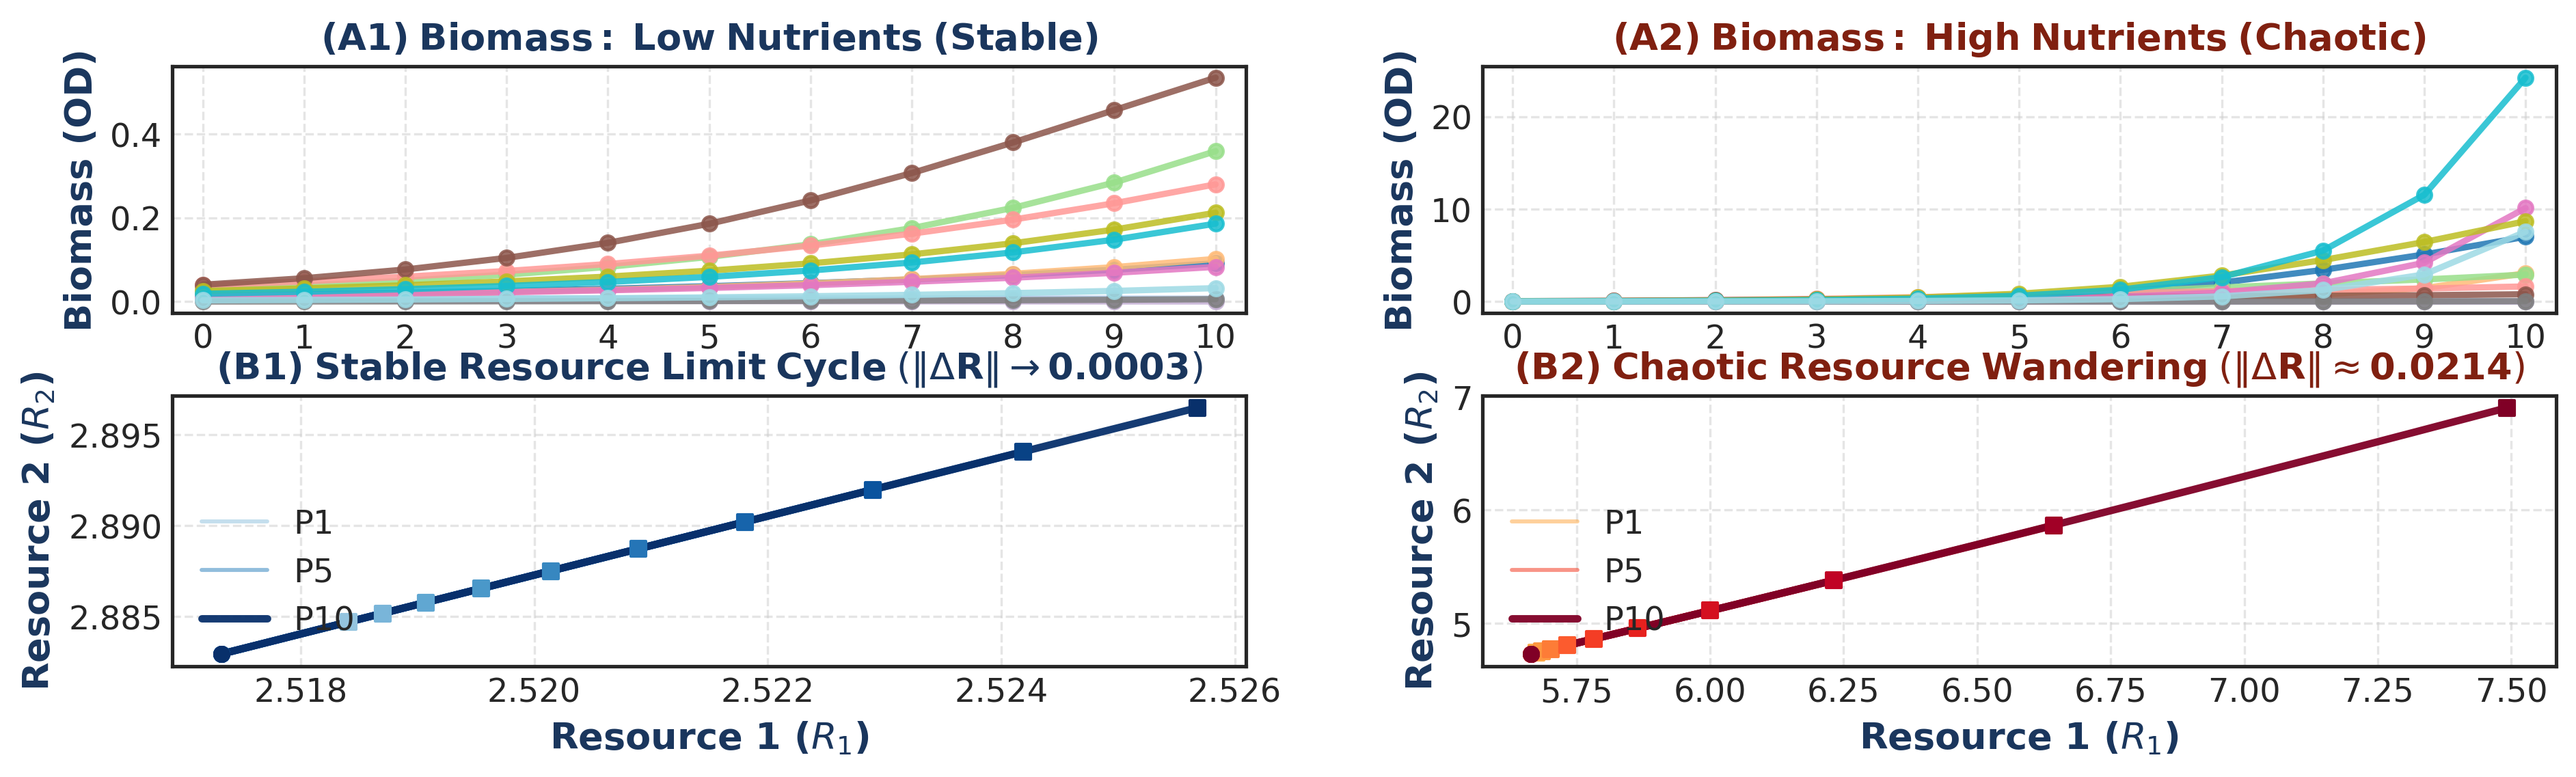
\includegraphics[width=0.98\linewidth]{figures/Gore_Phase_Space_Dynamics.png}
      \caption{\textbf{Stability vs. Chaos Driven Purely by Environmental Resources $\mathbf{R}_0$.} \textbf{(A1–A2)} Biomass dynamics $N_i(t)$ damping to a fixed point in LN vs. irregular oscillations in HN. \textbf{(B1–B2)} Multi-cycle resource trajectories $(R_1, R_2)$ converge onto an identical closed limit cycle in LN ($\|\Delta\mathbf{R}\| \to \mathbf{0.0003}$), but wander and diverge in HN ($\|\Delta\mathbf{R}\| \approx \mathbf{0.0214}$).}
    \end{figure}
  \end{block}

  % 7. EXPLORING MODEL EXTREMES: 24-SPECIES ENRICHMENT
  \begin{block}{7. Exploring Model Extremes: Taxonomic Biomarkers of Chaos}
    \begin{itemize}
      \item \textbf{Locked 100\% Recall Chaos Classifier:} Trained on $K=2$ physical trajectory features ($F_1 = 0.7458$, Recall = $100\%$, $T^* = 0.3891$). Correctly separates experimental $S=24$ communities in Medium Nutrients into stable and chaotic phases.
      \item \textbf{Chaotic Drivers (Sp 31–36, $+80\%$ in Chaos):} Generalists with balanced traits ($\theta_1 \approx \theta_2$) that concentrate competitive pressure in the niche center, driving chaos.
      \item \textbf{Stabilizing Specialists (Sp 37–42, $+80\%$ in Stable):} Extreme niche partitioners ($\theta_1/\theta_2 > 1.5$) that cleanly divide resources and enforce stability.
      \item \textit{Bacteria-agnostic random matrix models miss this taxonomic mechanism.}
    \end{itemize}

    \begin{figure}
      \centering
      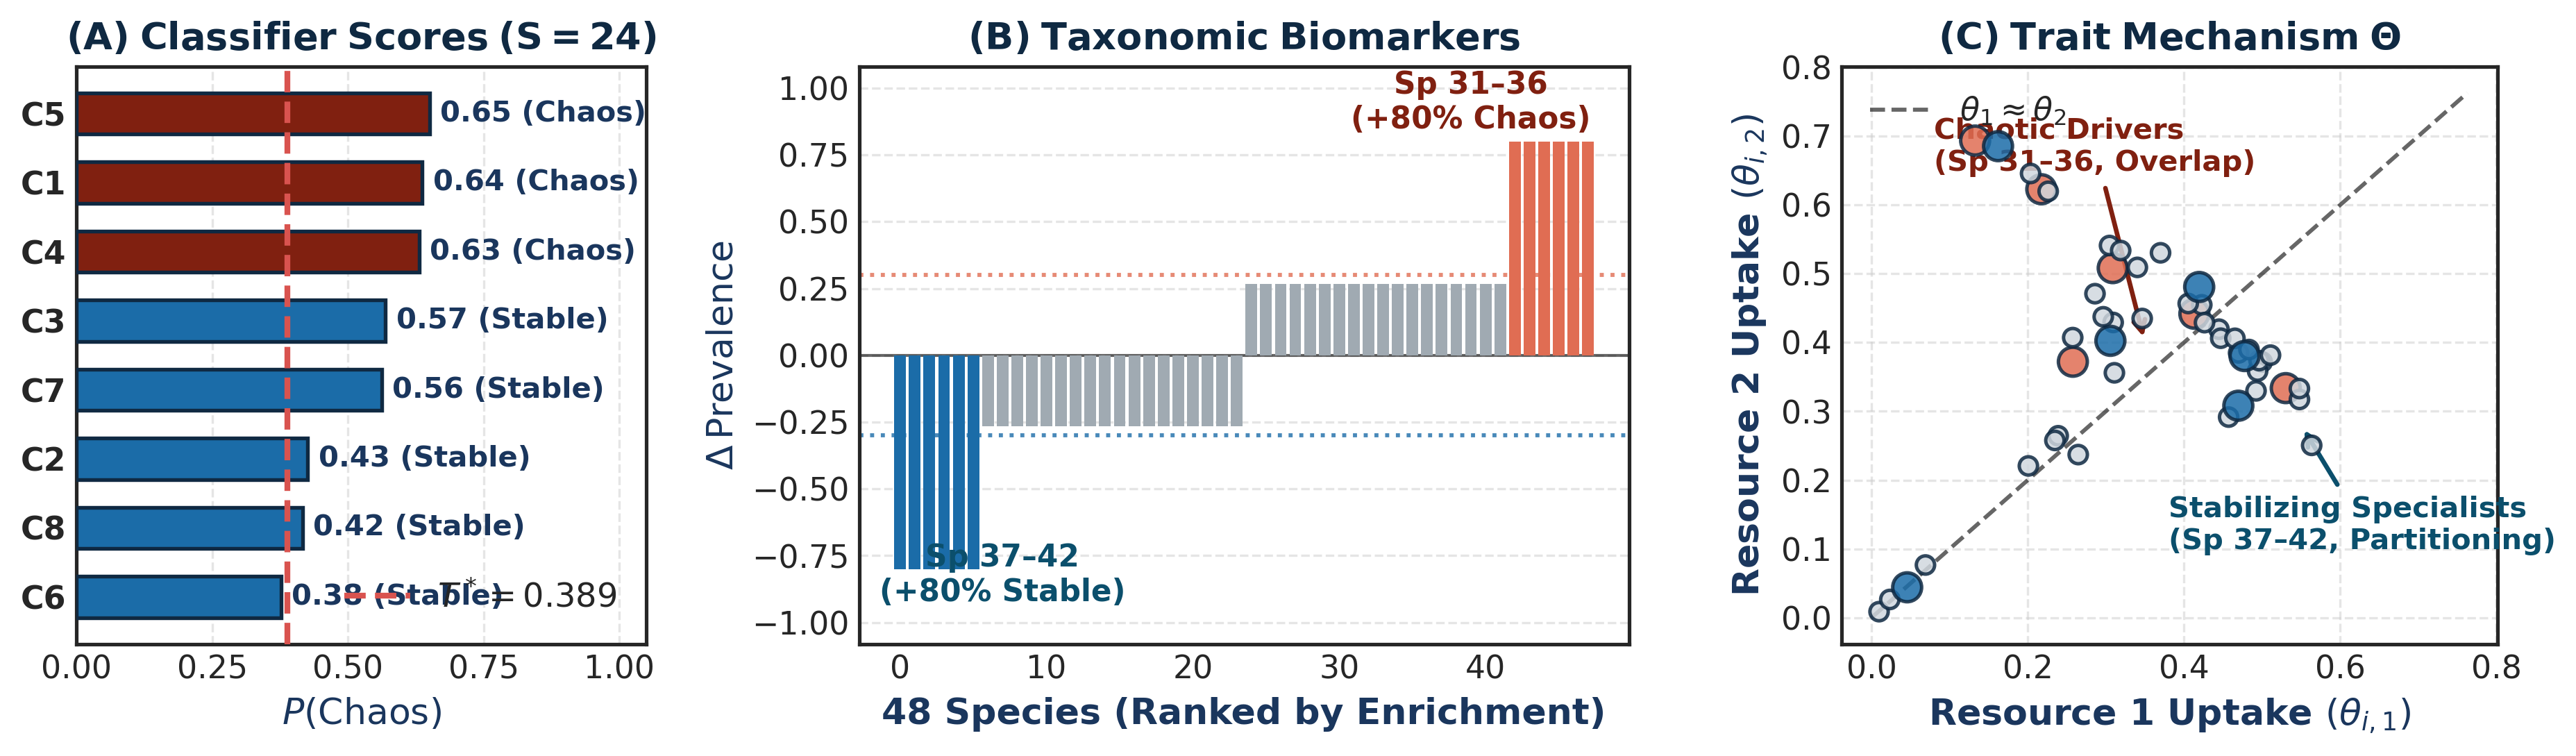
\includegraphics[width=0.98\linewidth]{figures/Gore_24Species_Enrichment.png}
      \caption{\textbf{Classifier Separation \& Taxonomic Biomarkers of Chaos.} \textbf{(A)} Classifier scores on experimental $S=24$ communities in MN. \textbf{(B)} Species enrichment $\Delta \text{Prevalence}$. \textbf{(C)} Metabolic trait map in $\mathbf{\Theta}$ space.}
    \end{figure}
  \end{block}

  % 8. KEY TAKEAWAYS & CONCLUSIONS
  \begin{block}{8. Key Takeaways \& Conclusions}
    \begin{enumerate}
      \item \textbf{Trait Universality:} Metabolic traits ($\mathbf{\Theta}$) and cross-feeding networks ($\mathbf{W}$) are universal biological invariants across spatial carriers and chemical perturbations ($R^2 = 0.72\text{--}0.97$).
      \item \textbf{Meaningful Environment Encoding:} Learned vectors $\mathbf{a}_c$ autonomously capture genuine environmental chemistry, outperforming null baselines and persistence models.
      \item \textbf{Deterministic Chaos \& Biomarkers:} Transitions between stability and chaos can be modulated purely by initial resources $\mathbf{R}_0$. Chaos is driven by symmetric niche generalists, whereas specialized resource partitioners enforce ecological stability.
    \end{enumerate}
  \end{block}

\end{minipage}\egroup\typeout{MEASURED_COL_HEIGHT: \the\ht0}

\separatorcolumn
\end{columns}
\end{frame}

\end{document}
